\section{Important Concepts}
\label{sec:concepts}

This section describes the definitions of the important concepts
regarding API usages and our representations.

\begin{figure}[t] %[!htp]
	\centering
	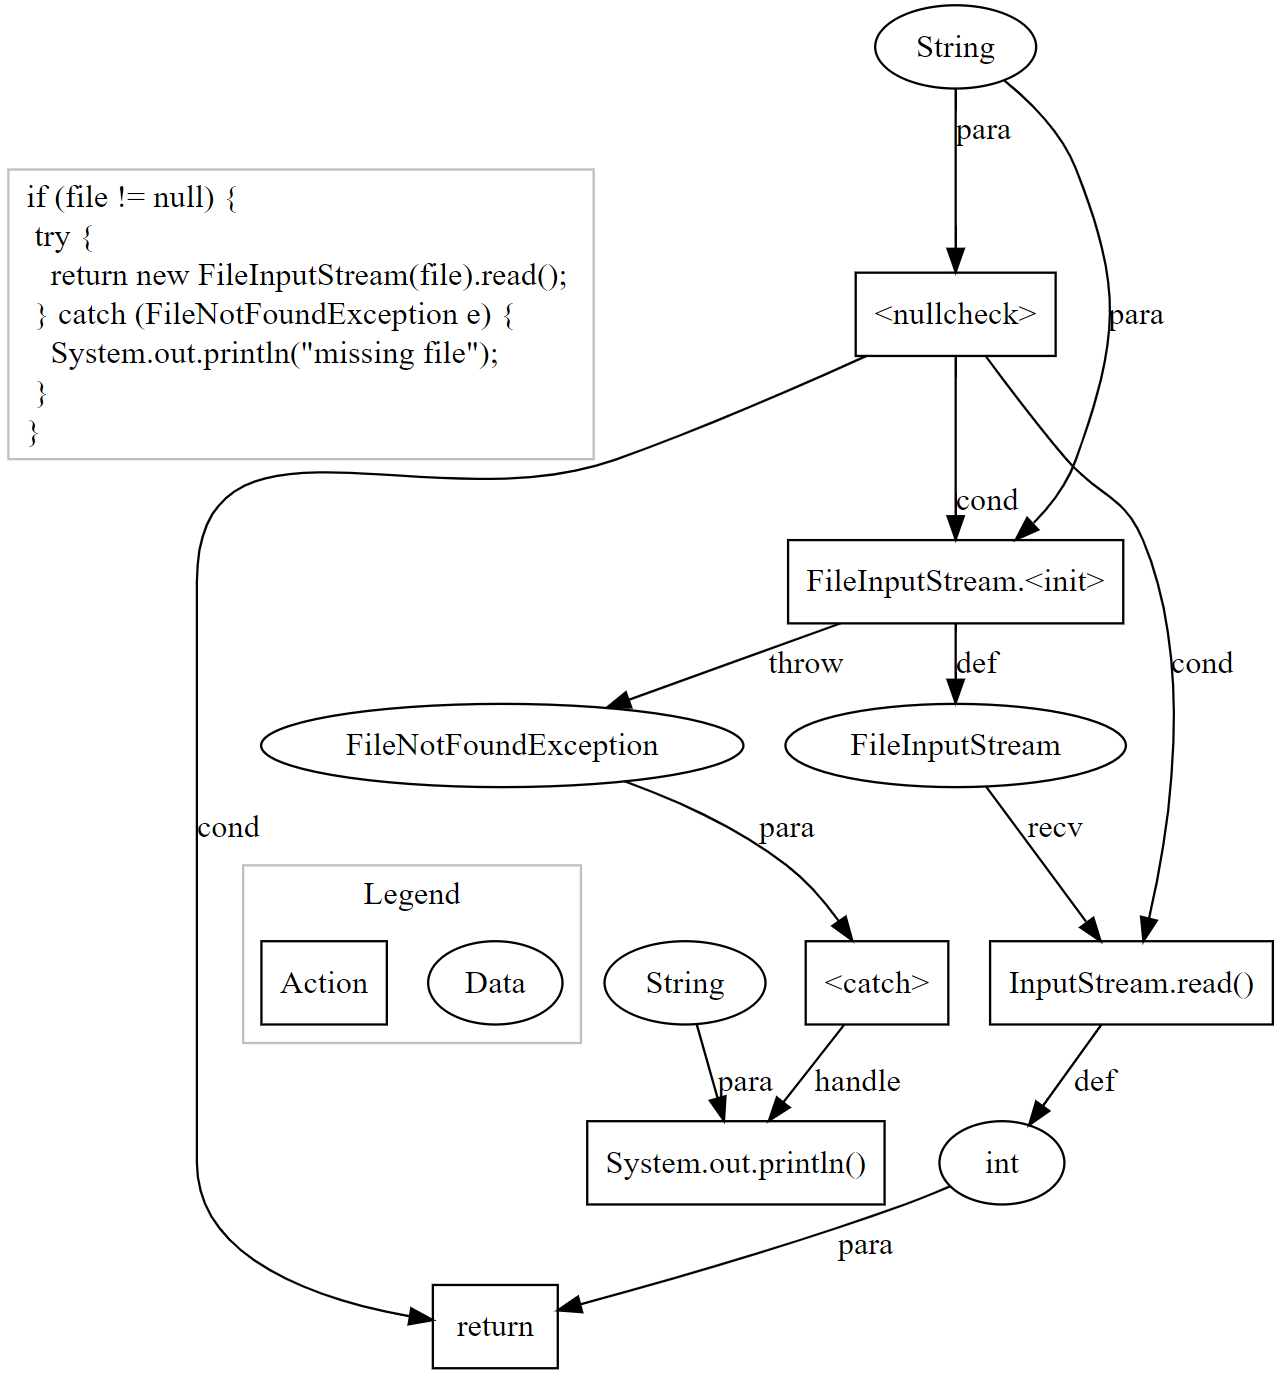
\includegraphics[width=0.9\linewidth]{aug-example}
        \vspace{-3pt}
	\caption{An API Usage and its API-Usage Graph}
	\label{fig:aug}
\end{figure}

\begin{Definition}[API elements]
  An API element is either a class, a method, or a field that is
  provided in a library to enable the accesses to the library's
  functions via a variable declaration with a certain class, a method
  call to an API method, or a field access to an API field.
\end{Definition}

For example, in Figure~\ref{fig:example3}, line 12, \code{Button} is
an API class, which is a declared type for the variable
\code{addStockButton}. At line 23, \code{addClickHandler} is an API
method, which is called on the variable \code{addStockButton}.

\begin{Definition}[API Usage]
An API usage consists of a set of API elements and control structures
(i.e., conditions and repetitions), together with other program
elements (e.g., variables, parameters, etc.) in specific combinations
and orders to perform a programming task.
\end{Definition}

In Figure~\ref{fig:example2}, lines 2-4 show an API usage consisting
of 1) a variable \code{myButton}, 2) its declared class \code{Button},
3) a method call to \code{addClickHandler} on the variable
\code{Button}, 4) the method call \code{addClickHandler} accepting an
argument of the type \code{ClickHandler}, etc.

\begin{Definition}[API Usage Relation]
  In an API usage, there exist the API usage relations among the API
  elements and relevant program elements. Those relations include
  receiver, parameter, definition, order, condition, synchronize,
  throw, and handle. They also include data and control dependencies.
\end{Definition}

Let us use the term {\em action} to refer to a method call, a field
access, or an operator. A {\em receiver} relation exists between a
variable and a method call. In Figure~\ref{fig:example2},
at line 3, there exists a receiver relation between the variable
\code{myButton} and the method \code{addClickHandler}. A {\em
  parameter} relation connects a variable to be used as a parameter of
an action. A {\em definition} relation exists between a constructor or
method call that creates or returns a value or object to the
respective variable. An {\em order} relation connects two actions on
operating on the same receiver or parameter. A {\em condition}
relation connects an action whose result controls branching to an
action being controlled. A {\em synchronize} relation connects a a
variable that the program obtains a lock on to an action executed
under that lock. A {\em throw} relation connects an action that may
throw an exception to a data node representing that exception
object. A {\em handle} relation connects from a \code{catch} action to
an action in a respective exception handling block.

We expect to leverage those API usage relations among the API elements
and relevant program entities to identify the FQNs. Toward that goal,
we adopt a graph-based representation for API usages, called {\em
  API-Usage Graphs (AUGs)}~\cite{msr19}.

\begin{Definition}[API Usage Graph (AUG)~\cite{msr19}]
AUG is a directed, connected graph with labelled nodes and
edges. Nodes represent data entities, such as variables, and actions,
such as method calls or operators. Edges represent the API usage
relations as well as control and data dependencies among entities and
actions represented by nodes.
\end{Definition}



Figure~\ref{fig:aug} shows an example of an API usage and its AUG.
The action nodes represent constructor calls (\code{init}), method
calls, field accesses, and operators. If the types are available, they
will be resolved. However, in the figure, only the simple name is
shown for clarity. The relational operators are also encoded as
actions to capture conditions. The data nodes represent objects,
values, and literals in an API usage. AUG encodes data entities as
nodes to make explicit the data dependencies between actions, such as
multiple calls on the same object to ensure we have a connected
subgraph with all data-dependent parts of a usage. The usage relations
are shown with their labels. The {\em order} edges are not shown for
clarity. Details on AUG and the building algorithm can be found
in~\cite{msr19}.
